\documentclass[10pt]{article}
% Packages
\usepackage{makecell} % For thicker lines
\usepackage{setspace}  % Controls line spacing
\usepackage{hhline}   % For double horizontal lines
\usepackage{colortbl}  % Add colour to LaTeX tables
\usepackage[T1]{fontenc}  % Choice of font encodings
\usepackage{tgtermes}  % Loads the TeX Gyre Termes font
\usepackage{siunitx}  % A comprehensive (SI) units package
\usepackage{tabularx, booktabs} % For advanced table layout
\usepackage{url}  % Verbatim with URL-sensitive line breaks
\usepackage{authblk}  % For author and affiliation management
\usepackage{natbib}  % A package for bibliographies and citations
\usepackage{graphicx}  % Enhances LaTeX's built-in graphics features
\usepackage{listings}  % Typeset programming code within the document
\usepackage{amssymb}  % Mathematical symbols
\usepackage[nottoc]{tocbibind}  % Adds entries to the table of contents
\usepackage{xcolor}  % Provides easy driver-independent access to colors
\usepackage{microtype}  % Improves the spacing between words and letters
\usepackage{enumitem}  % Control layout of itemize, enumerate, description
\usepackage{tocloft}  % Controls the typographic design of table of contents, etc.
\usepackage[breaklinks,linktocpage]{hyperref}  % Creates hyperlinks in your document
\usepackage[font=small,skip=7pt,labelfont=bf]{caption}  % Customising captions in floating envs

% Adjust the page margins in the bibliography
\let\oldthebibliography=\thebibliography
\let\endoldthebibliography=\endthebibliography
\renewenvironment{thebibliography}[1]{%
  \begin{oldthebibliography}{#1}%
    \raggedright%
    }{%
  \end{oldthebibliography}%
}

\setlength\bibindent{0pt}

% Optional options
% \usepackage{background} % Creates a DRAFT background image on all pages
% \backgroundsetup{contents=Preprint, opacity=0.25, color=gray} % Adds a watermark to the document
% This command changes the line spacing to double.
% ? Needed for reviews/drafts
% \doublespacing

% Custom colours
\definecolor{codegreen}{rgb}{0,0.5,0}
\definecolor{codegray}{rgb}{0.4,0.4,0.4}
\definecolor{codepurple}{rgb}{0.58,0,0.82}
\definecolor{backcolour}{rgb}{0.96,0.96,0.96}
\definecolor{lightgray}{gray}{0.8}

\lstdefinelanguage{JavaScript}{
  keywords={break, case, catch, continue, debugger, default, delete, do, else, finally, for, function, if, in, instanceof, new, return, switch, this, throw, try, typeof, var, void, while, with},
  morecomment=[l]{//},
  morecomment=[s]{/*}{*/},
  morestring=[b]',
  morestring=[b]",
  sensitive=true
}

% Listing styles
\lstdefinestyle{mystyle}{
  frame=tb,
  tabsize=2,
  captionpos=b,
  numbers=left,
  framerule=0pt,
  numbersep=5pt,
  showtabs=false,
  breaklines=true,
  keepspaces=true,
  showspaces=false,
  framextopmargin=6pt,
  framexbottommargin=6pt,
  showstringspaces=false,
  breakatwhitespace=false,
  keywordstyle=\color{purple},
  commentstyle=\color{codegreen},
  stringstyle=\color{codepurple},
  numberstyle=\tiny\color{codegray},
  basicstyle=\ttfamily\footnotesize,
  backgroundcolor=\color{backcolour}}
\lstset{style=mystyle}

% ! Custom template commands
% Add a vertical space after section numbers in ToC
\renewcommand\cftsecafterpnum{\vskip8pt}
% Changes the title of the list of listings
\renewcommand{\lstlistlistingname}{List of \lstlistingname s}
% Changes the title of the bibliography
\renewcommand{\bibname}{References}
% Changes the title of the table of contents
\renewcommand{\contentsname}{Table of Contents}
% Changes the leader between section and page numbers in ToC
\renewcommand{\cftsecleader}{\cftdotfill{\cftdotsep}}
\newcommand{\floatcaption}[2]{\caption[#1.]{#1~#2.}}

% Custom template settings
\captionsetup{justification=centering}  % All captions will be centered
\hypersetup{
  colorlinks = true,
  urlcolor = blue,
  linkcolor = blue,
  citecolor = blue,
  breaklinks = true
}
\PassOptionsToPackage{hyphens}{url}
\urlstyle{same}
\def\Urlmuskip{0mu plus 1mu}
\def\UrlBreaks{\do\/\do-}
\def\UrlBigBreaks{\do\/\do-\do:\do.}
\setlist[itemize]{noitemsep, topsep=0pt, partopsep=0pt}



\begin{document}
% Changing the initial page numbering to uppercase Roman
\pagenumbering{roman}
% Resetting the page counter to 1
\counterwithin{lstlisting}{section}
\counterwithin{figure}{section}
\counterwithin{table}{section}
% Sets the distance between the bottom and the footer
\setlength{\footskip}{65pt}

% ! ===============================
% ! Start of the title page content
% ! ===============================

\title{\textbf{WebAssembly and the \linebreak  Wizards of Hogwarts}}
\author[1]{Daniel Burger}
\affil[1]{\textbf{Middlesex University London\thanks{In collaboration with SAE Institute Zürich.}}}
\affil[ ]{\href{mailto:public@danielburger.online}{public@danielburger.online}}
\date{\textit{7. November 2020}}
\maketitle
% Resetting the page style for the first page
\thispagestyle{empty}

% The sloppypar environment adjusts the spaces between words such that each line fits into the text width
\begin{sloppypar}
  \begin{abstract}
    There is a new kind in the web development hood: WebAssembly. It is fast, portable, supported by the big players, and should allow the World Wide Web to become the largest software platform in existence. It does not matter if a person is an experienced software engineer or a beginner web developer—everyone can profit from WebAssembly’s existence.

    In this essay, we will look at what WebAssembly is, how it works and how it works alongside its sibling JavaScript.
  \end{abstract}

  \pagebreak
  % Changing the page numbering back to uppercase Roman
  \pagenumbering{Roman}
  \tableofcontents
  \pagebreak
  \listoffigures
  \pagebreak
  \listoftables
  \pagebreak
  \addcontentsline{toc}{section}{\lstlistlistingname} % Add to the TOC
  \lstlistoflistings
  \pagebreak
  % Changing the page numbering back to Arabic
  \pagenumbering{arabic}

  % ! ====================================
  % ! Start of the actual document content
  % ! ====================================

  \section{Introduction}
  \label{sec:introduction}

  On the 17th of June 2015, Brendan Eich—the inventor of JavaScript—and the teams behind Mozilla, Chrome, Edge and WebKit presented a new browser standard: \mbox{WebAssembly}, a portable and highly efficient byte-code compilation target for high-level languages such as C++ and Rust \citep{eich_asmjs_2015}.

  However, what does this mean? What is the reason that WebAssembly should exist in the first place? Should JavaScript developers be worried now? Furthermore, what do the wizards of Hogwarts have to do with it?

  \subsection{Web Development Back Then}
  \label{sec:back-then}

  Back in the day, when people could call themselves web developers because they only understood HTML, web development was a rather interactionless and static field of business. Netscape Communications, a pivotal company in the development of the modern web and the creator of the Netscape Browser (shown in \autoref{fig:netscape}), quickly recognised that websites of the time lacked interactivity and dynamism. They wanted the web to be a new form of a distributed operating system rather than just a simple HTML document-accessing application on people’s computers \citep{cassel_brendan_2018}.

  \begin{figure}[ht]
    \centering
    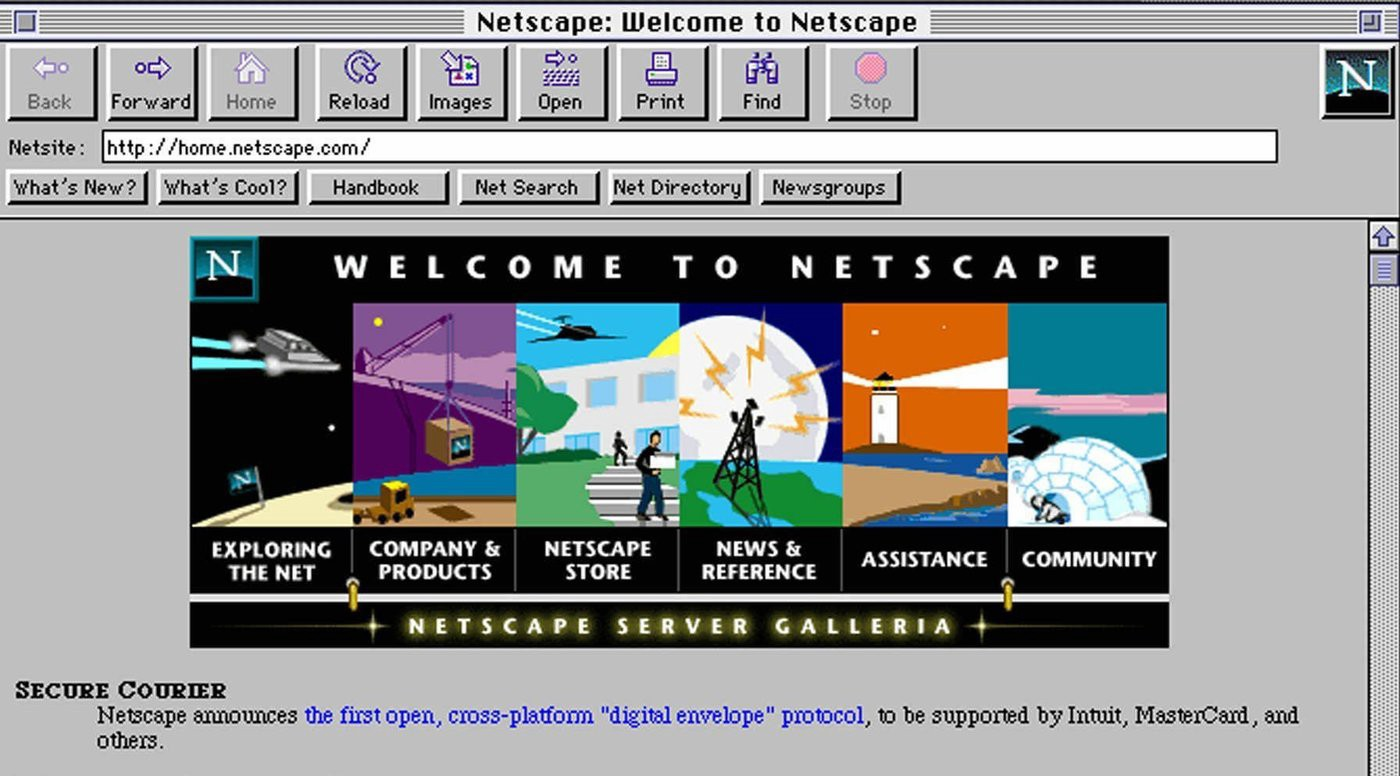
\includegraphics[width=\textwidth]{figures/netscape.jpg}
    \floatcaption{Screenshot of the Netscape browser and start-page}{\citep{npr_home_nodate}}
    \label{fig:netscape}
  \end{figure}

  Marc Andreessen, founder of Netscape Communications, proposed that HTML needed some kind of “scripting language” that was approachable, something you could glue directly into the markup. A language that is easy to use by newbie programmers who do not want to handle compiler errors or strictly typed syntax.

  That was why they hired the experienced programming language and network developer Brendan Eich. Brendan’s first task was the nearly unachievable goal of creating such a scripting language for the web—due in 10 days. They (later) called it JavaScript \citep{severance_javascript_2012}.

  \subsection{JavaScript’s Destiny}
  \label{sec:javascript-destiny}

  One does not need to dig too deep into the history of the web to show one crucial pain point of today’s web technology standards: JavaScript is a scripting language for the browser to interpret—not some fancy multi-paradigm system programming language that focuses on speed, security or code maintainability. It was supposed and designed to be an easy-to-understand dynamically typed scripting language to, e.g. give a website fast DOM manipulations and decorative animations.

  Nevertheless, see what happened:

  \begin{quote}
    \emph{“Any application that can be written in JavaScript will eventually be written in JavaScript.” \citep{atwood_principle_2007}}
  \end{quote}

  This is a quote by Jeff Atwood (co-founder of Stack Exchange), commonly referred to as Atwood’s Law. Ever since frameworks like Node.js or React Native became widely used, JavaScript’s possibilities have already crossed the border of just living on the client side inside of a browser. It is nearly everywhere.

  Also, Node.js’ NPM package manager is currently the most prominent and active package registry platform ever created. As an example: From the 10th of May to the 17th of May of 2018, JavaScript developers downloaded 5.2 billion Node.js packages from the NPM registry, setting a new record \citep{npm_how_2018}

  \begin{figure}[ht]
    \centering
    \frame{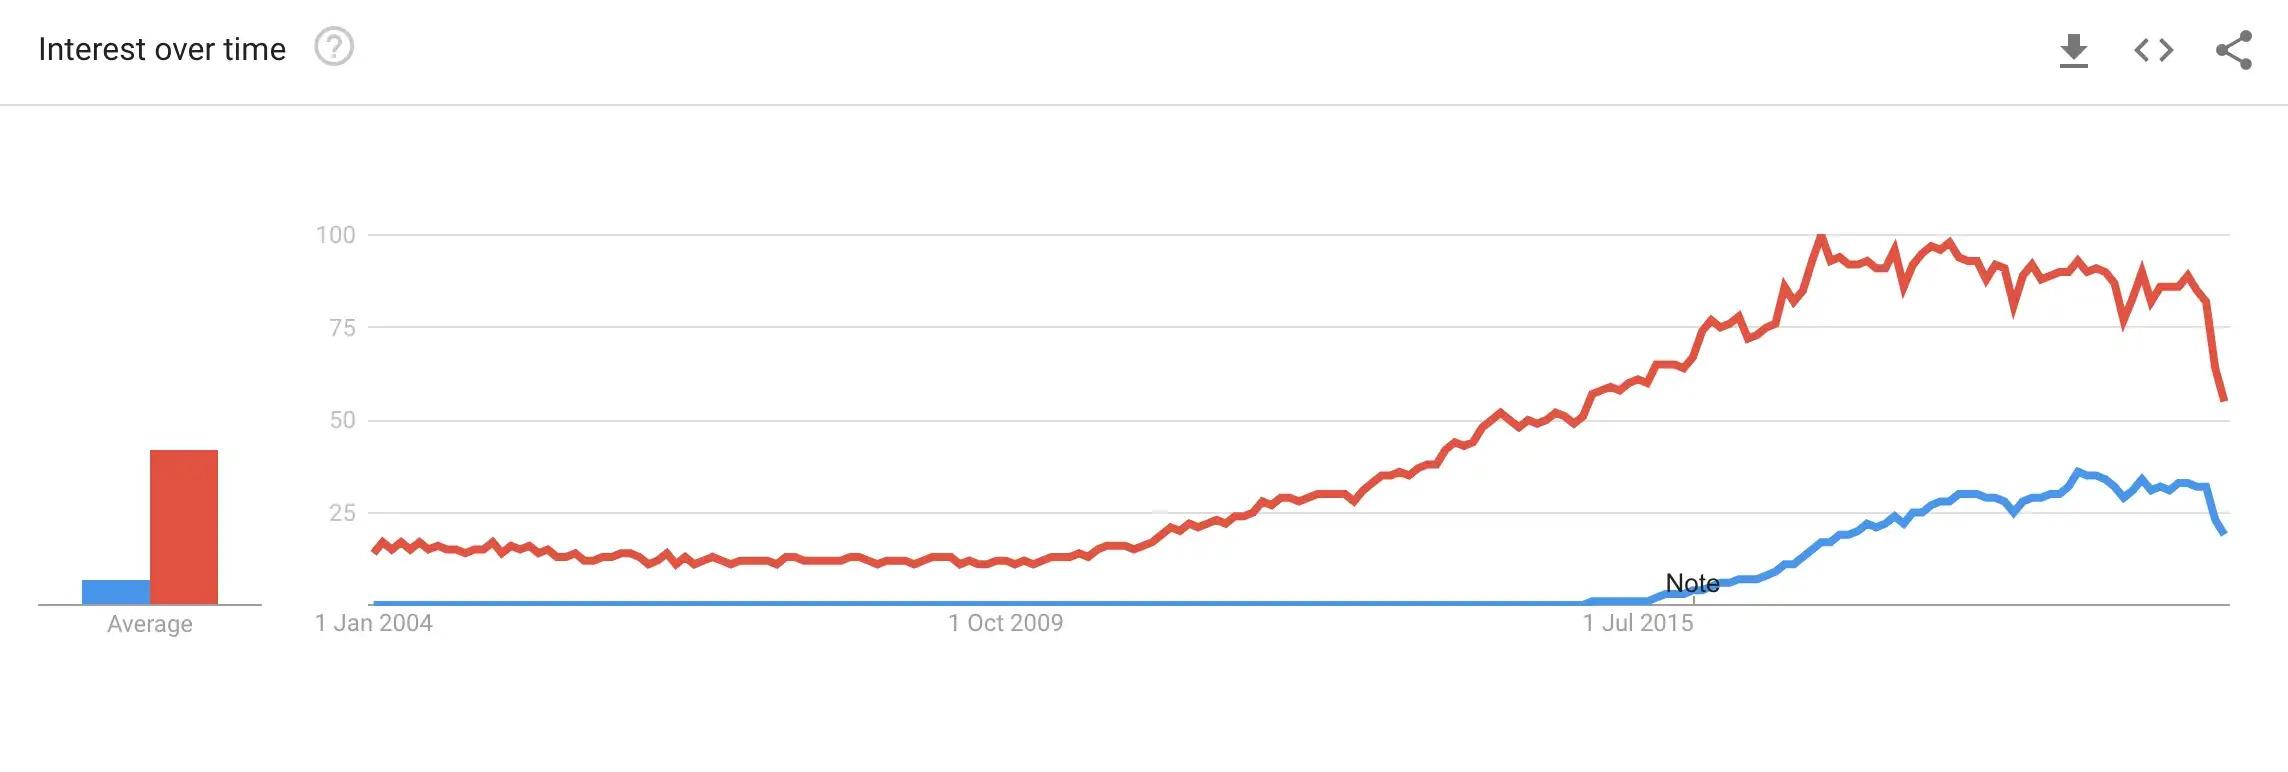
\includegraphics[width=\textwidth]{figures/google-trends.jpg}}
    \floatcaption{Google Trends curve about Node.js and React Native}{\citep{google_google_nodate}}
    \label{fig:atwood-law}
  \end{figure}

  \subsection{Treacherous Atwood’s Law}
  \label{sec:atwood-law}

  There are thousands of courses, books and tutorials on how to learn JavaScript. Every computer-related school now or then teaches JavaScript. Nearly everyone can learn it anywhere with a minimum amount of effort. The search term for “Learn JavaScript” on Google will get \num{2220000000} search results. In comparison, the search term “Learn Java” will get \num{305000000} results.

  Though, is that a good thing? Is an originally lightweight scripting language capable of ruling the world of computational web development? My opinion: No, it is not, and there will not be such a bright future for JavaScript as nearly everybody claims. Let me explain it with a Harry Potter analogy:

  \subsection{Muggles Entering Hogwarts}
  \label{sec:muggles}

  Do you know how it feels to watch web developers call themselves “full-stack software engineers” after they have simply learned Node.js? It feels like Muggles entering Hogwarts—a school full of wizards. Only in our case, these wizards are trained software engineers and computer scientists. These are the people who learn and work on all the hardcore-implemented algorithms and compilers, programming languages and operating systems. They know precisely how to build software \citep{might_what_2011}. Do web developers know how to write actual software? I would say we better not talk about it.

  Muggles are not invited to Hogwarts because they have no magical ability. Web developers were not “invited” to software engineering, too, because they could not even do something with the languages they knew. What they wrote was not even considered software per se, just web pages. Nevertheless, thanks to all the cross-platform JavaScript runtimes, they are suddenly here to do some magic. However, imagine what if the wizards of Hogwarts, our beloved software engineers and computer scientists, could perform magic in the real world—or, in our case, the web? What would happen? What could go wrong?

  \section{WebAssembly Says Hello World}
  \label{sec:hello-world}

  WebAssembly is the new player in the web development industry. It is fast, small, non-readable and not even an actual programming language. You literally cannot code in WebAssembly \citep{rourke_learn_2018}. So, why should we all be excited about it? As mentioned earlier, it is a compilation byte-format target for high-level languages.

  \begin{figure}[ht]
    \centering
    \frame{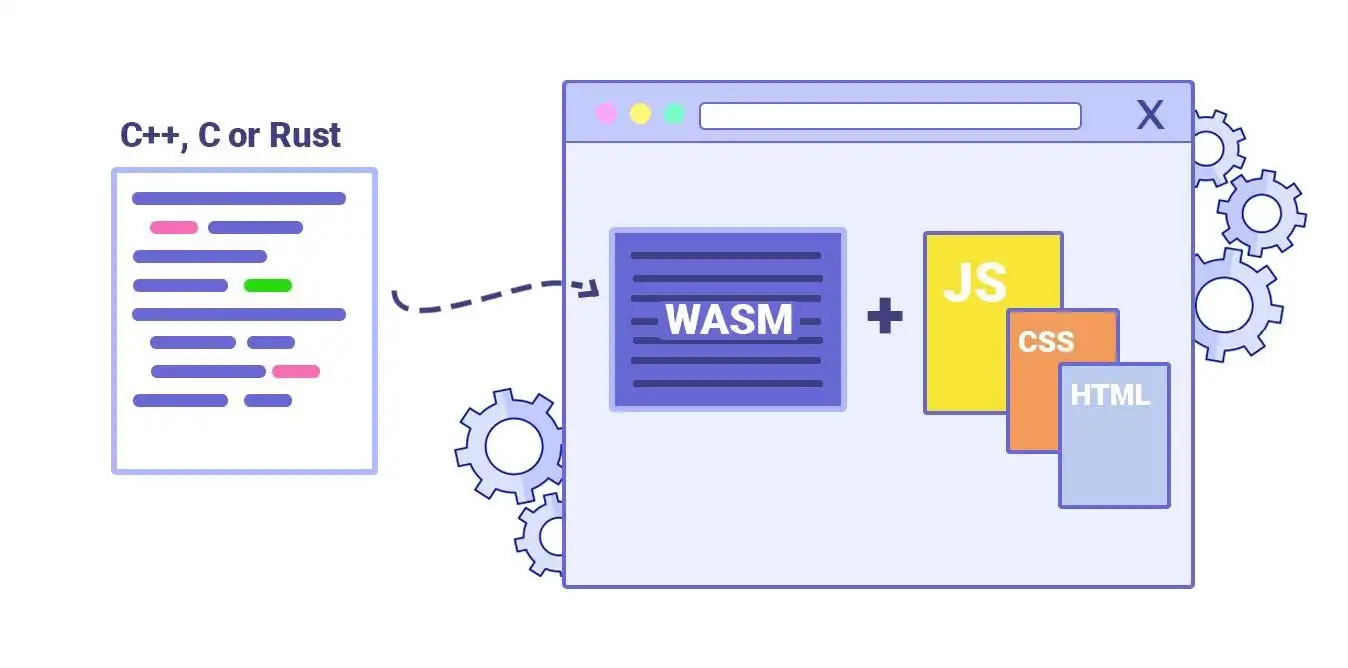
\includegraphics[width=\textwidth]{figures/wasm.jpg}}
    \floatcaption{Illustration of how WebAssembly modules are being delivered to the browser}{\citep{logrocket_logrocket_nodate}}
    \label{fig:wasm}
  \end{figure}

  You write your code in a high-level language like C or C++ and compile it to WebAssembly. The magic trick: It works in the browser and is super fast—sometimes about 5 to 20 times faster than JavaScript \citep{aboukhalil_how_2019}.

  \section{WebAssembly in a Nutshell}
  \label{sec:wasm-in-a-nutshell}

  The real face behind the term “WebAssembly” is not as uniform as it is being marketed. WebAssembly itself is only a piece of a bigger technology chain of workflows and concepts. Several other key components are essential for delivering super-fast web applications. It is also good to know its current limitations and which use cases it is the best for. Nevertheless, first, let us talk about the five key components:

  \subsection{WAT~—~WebAssembly Text Format}
  \label{sec:webassembly-text-format}

  This is a human-readable file format you will get when you compile your C, C++ or Rust code. It represents the abstract syntax tree (AST) from the source code of a programming language. An AST—or, in the WebAssembly case, a .wat file—may be verbose, but it does an excellent job describing the source code components. Representing source code in an AST makes verification and compilation simple and efficient. Here is a simple return function called \lstinline{getDoubleNumber} written in C:

  \vspace{7pt}
  \begin{lstlisting}[language=C, caption=Code example in C., label=lst:c-example]
  int getDoubleNumber(int x) {
    return x * 2;
  }\end{lstlisting}

  Compiling this C code will return a \lstinline{.wat} file containing the abstract syntax tree of our \lstinline{getDoubleNumber} function. It looks like this:

  \vspace{7pt}
  \begin{lstlisting}[language=C, caption=Code example from above compiled into the WebAssembly Text Format., label=lst:wat-example]
  (module
    (table 0 anyfunc)
    (memory $0 1)
    (export "memory" (memory $0))
    (export "getDoubleNumber" (func $getDoubleNumber))
    (func $getDoubleNumber (; 0 ;)
      (param $0 i32) (result i32)
    (i32 .shl
      (get_local $0)
      (i32.const 1)
      )
    )
  )\end{lstlisting}

  \subsection{WASM~—~WebAssembly Binary Instruction Format}
  \label{sec:webassembly-binary-instruction-format}

  While in production, you probably will not send the text instruction format file to the client side. You will only send the binary instruction format (.wasm). This is the actual low-byte format file, written in non-readable hexadecimal code. Usually, they are referenced as WebAssembly modules \citep{mozilla_webassembly_2023}. Here is the example from the \lstinline{getDoubleNumber} C function from above:

  \vspace{7pt}
  \begin{lstlisting}[language=C, caption=Code example from above compiled into the WebAssembly \\ Binary Instruction Format., label=lst:binary-example]
  0061 736d 0100 0000 0186 8080 8000 0160 017f 017f 0382
  8080 8000 0100 0484 8080 8000 0170 0000 0583 8080 8000
  0100 0106 8180 8080 0000 079c 8080 8000 0206 6d65 6d6f
  7279 0200 0f67 6574 446f 7562 6c65 475 6d62 6572 0000
  0a8d 8080 8000 0187 8080 8000 0020 0041 0174 0b\end{lstlisting}

  \subsection{WASM Module Instantiating}
  \label{sec:webassembly-module-instantiating}

  If you want to access the C code within your website, you need to instantiate the WebAssembly .wat module inside JavaScript. This would look like this:

  \vspace{7pt}
  \begin{lstlisting}[language=JavaScript, caption=Instantiate the .wasm module in JavaScript., label=lst:javascript-example]
  // Access the WebAssembly object
  WebAssembly.instantiateStreaming(
    fetch("program.wasm"), imports)
    // Resolve the promise
    .then(_wasm => {
      // Log something if it worked
      console.info("WASM is ready")
    })\end{lstlisting}

  \subsection{WebAssembly Compilation}
  \label{sec:webassembly-compilation}

  In order to get a .wasm or .wat file, you first need to compile your source code. There are already different compilers for the various languages out there. The most common one—and also the most famous one—is called Emscripten. Emscripten is described as a so-called LLVM source-to-source compiler with the main focus of compiling C code straight to a subset of JavaScript known as asm.js. However, the recent rise of WebAssembly has pushed the team behind Emscripten to shift its focus to help make WebAssembly more accessible and easier to start with. You can then access the Emscripten compiler inside your command-line interface to easily compile selected source code.

  \subsection{Original Source Code}
  \label{sec:original-source-code}

  To write efficient software and compile it to WebAssembly, you must be proficient in C, C++ or the Rust programming language (or use AssemblyScript if you are familiar with TypeScript). The WebAssembly Working Group has plans to add more languages in the near future. However, they have other priorities and next steps on their roadmap. They primarily focus on the most significant pain points of WebAssembly.

  \section{Pain Points And Limitations}
  \label{sec:pain-points-and-limitations}

  The WebAssembly workflow sounds too good to be true. Just write your code in a high-level language, compile it via Emscripten, and then instantiate it inside JavaScript—it is as easy as that. Well, no, it is not. There are still some considerable pain points for easily porting your desktop-like application to the web despite not having a garbage collector or exception handlers \citep{w3c_roadmap_2019}. The most significant pain point right now is, for sure, the lack of web APIs. Let us say you want C++ code that can listen if a user clicks a button and then render some data from your database into the client-side DOM view.

  Well, I need to disappoint you; this will not work because WebAssembly cannot access the DOM API. The only way to access it is via JavaScript. If you want to develop actual WebAssembly-ready client-side software, you would need to write some JavaScript glue code \citep{mihaylov_how_2018} that acts as the asynchronous bridge between your WASM module and the client-side HTML page.

  \begin{figure}[ht]
    \centering
    \frame{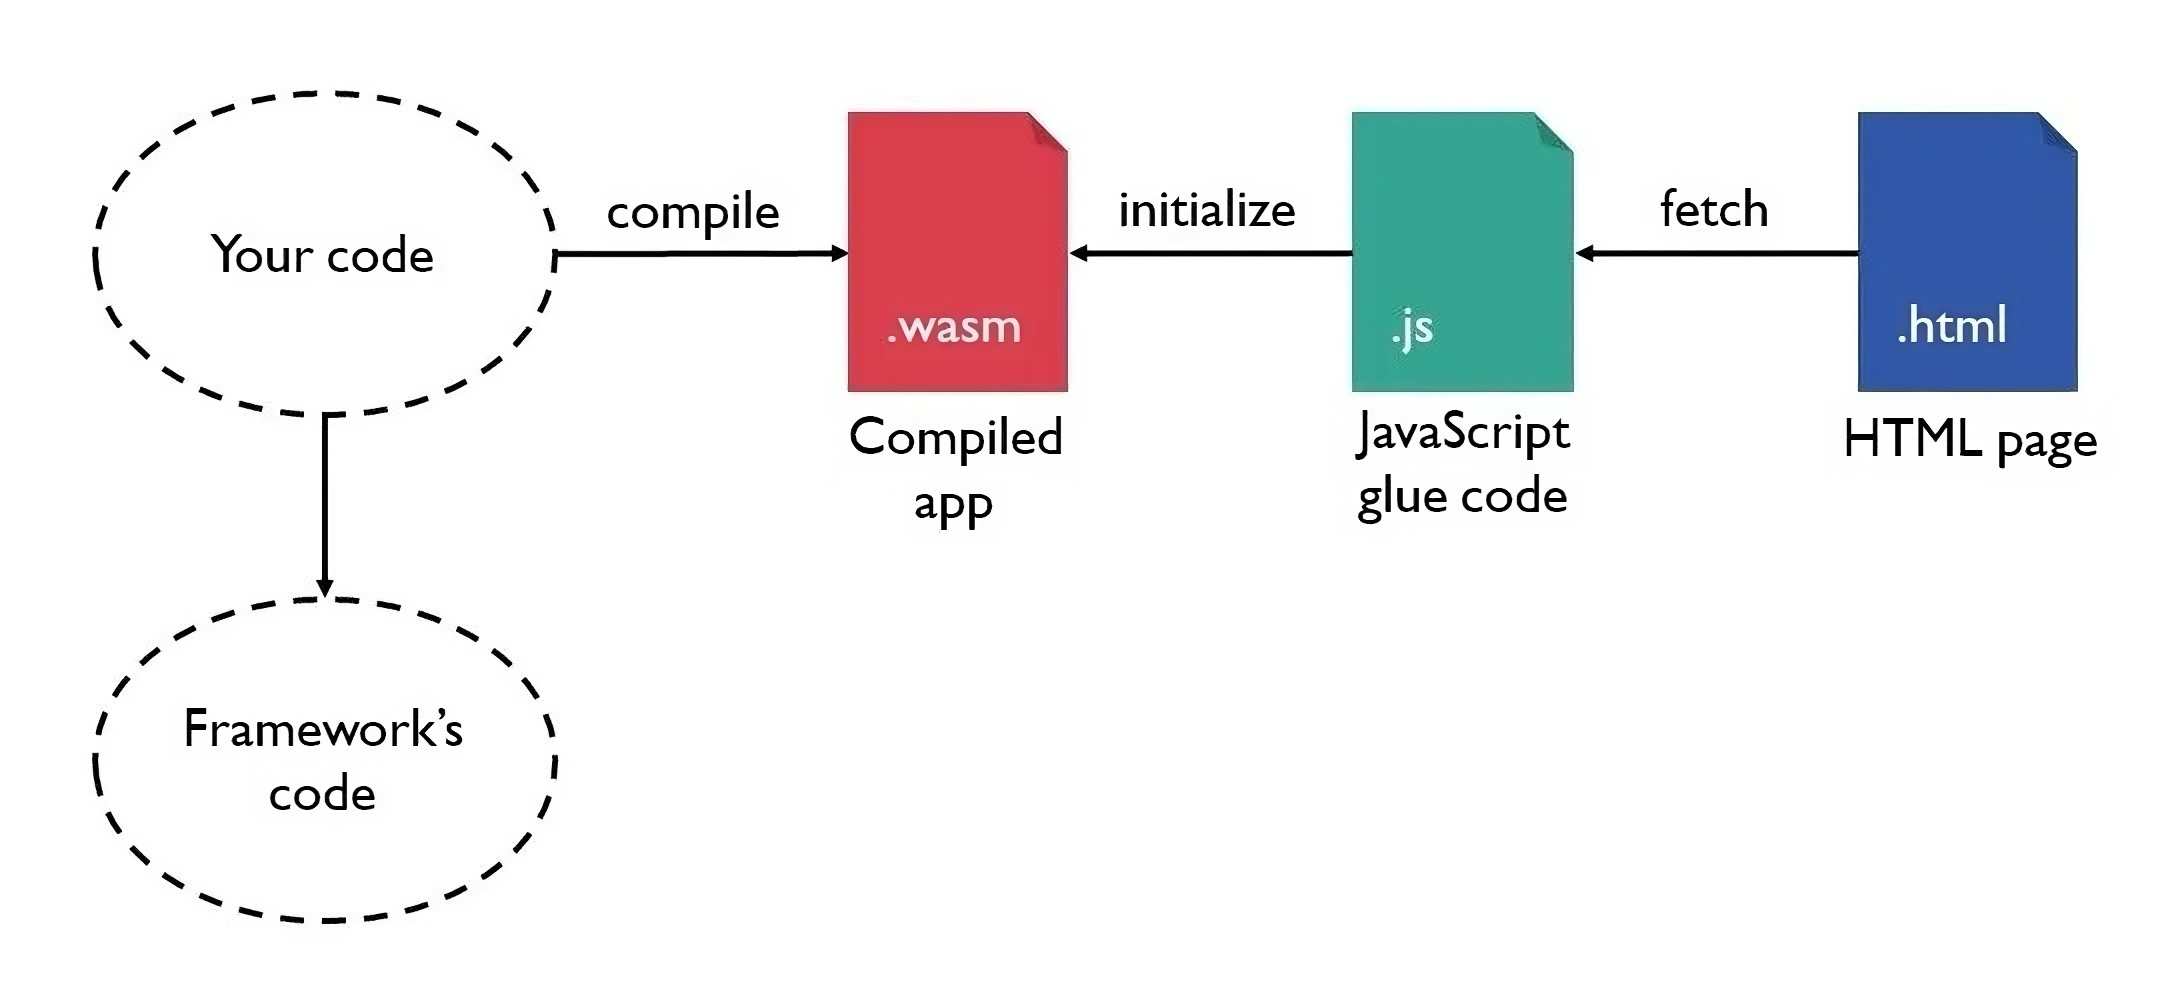
\includegraphics[width=\textwidth]{figures/glue-code.jpg}}
    \floatcaption{Illustration of how WebAssembly works together with JavaScript}{\citep{mihaylov_how_2018}}
    \label{fig:glue-code}
  \end{figure}

  \section{Current Best Use Case}
  \label{sec:use-cases}

  As of today, the best use case for WebAssembly under these circumstances is math-heavy calculations for graphics rendering inside an HTML5 canvas element. The canvas element is the only place to create a graphical user interface without accessing the DOM. This does not sound very interesting to many, but at least it is super promising for the gaming industry. Since games rely on computationally heavy shader calculations and simulations, compiling WebAssembly makes perfect sense. That is why Epic Games showcased a compiled Unreal Engine C++ high-resolution game inside the browser. Everything related to high-fidelity graphics or simulations is the most straightforward fit for WebAssembly right now—but for everything else that still needs to access or manipulate the DOM, use a glue code mixture between WebAssembly and JavaScript.

  \section{Glue Code}
  \label{sec:glue-code}

  But wait, this sounds familiar? Glue code? Wasn’t this the original purpose of JavaScript? Well, yes, it was. However, since the WebAssembly Working Group is actively working on an official DOM API \citep{mozilla_webassemblymodule_2023}, what is the primary purpose of JavaScript in the first place? If we can soon create very efficient full-stack web applications with just one high-level language, do we really need JavaScript in the near future?

  Well, we do not know; you cannot kill a whole ecosystem with millions of developers overnight. This did not work for PHP and will not work for JavaScript either. However, different people have different predictions. Moreover, the following chapter describes some predictions for the future.

  \section{WebAssembly's Future}
  \label{sec:webassembly-future}

  Since people with in-depth knowledge of software development and computer science—aka our Wizards from Hogwarts — soon have the ability to port their power to the client side, we will most likely see a completely new age of the World Wide Web as we know it today. Netscape Communications’ original vision of the web as a distributed operating system could finally become a reality. Native apps and their app stores are going extinct, and whole software packages like the suites from Adobe and Autodesk will run entirely inside the browser. The web will push its borders far beyond what we now define as the information and entertainment industry epicentre.

  In the future, JavaScript will still have an essential role, but not as crucial as today. It will act as a simple scripting language to provide websites with dynamic content and to create animations. The positioning of JavaScript will most likely be like the one it initially was being created for, and WebAssembly will act as the binary format for the browser to do all software-like heavy-lifting as, e.g. the real-life uses cases in \autoref{tab:use-cases} present.

  \begin{table}[ht]
    \centering
    % Increasing space between rows
    \renewcommand{\arraystretch}{1.5}
    % Increasing space between columns
    \renewcommand{\tabcolsep}{7pt}
    \begin{tabularx}{\textwidth}{{@{}lX@{}}}
      \Xhline{2.75\arrayrulewidth} % Makes the top line thicker
      \textbf{Company}  & \textbf{Use Case}                                                                                                                                                                    \\
      \midrule
      \textbf{Figma}    & Browser-Based Interface Design Tool. Initially, it was written in C++ and compiled from C++ to asm.js. Switching to WebAssembly improved document loading times by over three times. \\
      % Start coloring the lines light gray
      \arrayrulecolor{lightgray}
      \midrule
      \textbf{Autodesk} & CAD Drawing Software. Autodesk AutoCAD’s original code, older than the WWW, was compiled into WebAssembly as a web app.                                                              \\
      \midrule
      \textbf{eBay}     & Barcode Scanner. eBay improved their JavaScript barcode scanner by rebuilding it in C++ and compiling it to WebAssembly to enhance its success rate significantly.                   \\
      % Revert the rule color back to black
      \arrayrulecolor{black}
      \addlinespace
      % Makes the top line thicker
      \Xhline{2.75\arrayrulewidth}
    \end{tabularx}
    \caption{Real-life use cases for WebAssembly}
    \label{tab:use-cases}
  \end{table}

  % ! ==============================================
  % ! Start of the references and appendices content
  % ! ==============================================

  \pagebreak
  \bibliographystyle{../../templates/custom-apa}
  \bibliography{references/bibliography}

\end{sloppypar}
\end{document}
